% context: 9th-grade physics problem set, mechanical advantage
% topic: pulleys, levers, chain/trig, hydraulics; unit conversion + circle geometry
\documentclass[12pt, twoside]{article}
\input{../preamble}
\usepackage{float}
\usetikzlibrary{angles, quotes}

\title{Physics}
\author{Chris Huson}
\date{May 2026}

\fancyhead[LE]{\thepage}
\fancyhead[RO]{\thepage \\ First \& last name: \hspace{2.25cm} \,\\ Grade: \hspace{2.25cm} \,}
\fancyhead[LO]{La Scuola d'Italia / Huson / Physics \\* 29 May 2026}

\begin{document}

\subsubsection*{3.6 Problem Set: Mechanical Advantage}

\textbf{Formulas (provided).} \quad
$\text{MA} = \dfrac{F_\text{out}}{F_\text{in}}$ \qquad
Pulley (ideal): MA $=$ number of supporting strands \qquad
Lever: MA $= \dfrac{\text{effort arm}}{\text{load arm}}$

\smallskip
Pressure $P=\dfrac{F}{A}$; \; Pascal: $\dfrac{F_1}{A_1}=\dfrac{F_2}{A_2}$ \qquad
Circle area $A=\pi r^2$ \qquad
Chain at midpoint: $F_\text{pull}=2\,T\sin\theta$

\smallskip
$1~\text{Pa}=1~\text{N/m}^2$ \quad $1~\text{kPa}=1000~\text{Pa}$ \quad $1~\text{PSI}=6.895~\text{kPa}$ \quad $g=9.8~\text{m/s}^2$

\hrule
\vspace{0.3cm}

\begin{enumerate}[itemsep=0.45cm]

%--- Problem 1: pulleys (fixed, movable, block-and-tackle) ---
\item \textbf{Pulleys.} A warehouse worker lifts crates with three pulley setups.
  \begin{enumerate}[itemsep=2.7cm]
    \item State the ideal mechanical advantage of a single \emph{fixed} pulley, and say what it is good for.
    \item A single \emph{movable} pulley supports a $240~\text{N}$ load on two strands. What effort force ideally lifts it?
    \item A block and tackle has $4$ strands supporting the load. Find the ideal effort force to lift a $600~\text{N}$ crate, and the length of rope you must pull to raise the crate $0.50~\text{m}$.
  \end{enumerate}
  \vspace{1.3cm}
\newpage
%--- Problem 2: lever ---
\item \textbf{Lever.} A steel bar is used as a lever to lift a $850~\text{N}$ rock. The fulcrum sits $0.20~\text{m}$ from the rock (load arm); you push down at a point $1.20~\text{m}$ from the fulcrum (effort arm).
  \begin{enumerate}[itemsep=4.7cm]
    \item Find the ideal mechanical advantage.
    \item Find the effort force needed to balance the rock (ideal case).
    \item You push the long end down $0.30~\text{m}$. How far does the rock rise? Comment on the trade-off.
  \end{enumerate}
  \vspace{1.3cm}

  \newpage
%--- Problem 3: chain pulled laterally (trig MA) ---
\item \textbf{Chain and stuck car.} A chain is stretched tight and straight between a tree and a car
stuck in a ditch. You pull \emph{sideways} at the midpoint with a force $F_\text{pull}=300~\text{N}$,
deflecting the chain by $\theta = 10^\circ$ from the straight line. The sideways pull is balanced by the
two chain tensions: $F_\text{pull}=2\,T\sin\theta$.

\begin{center}
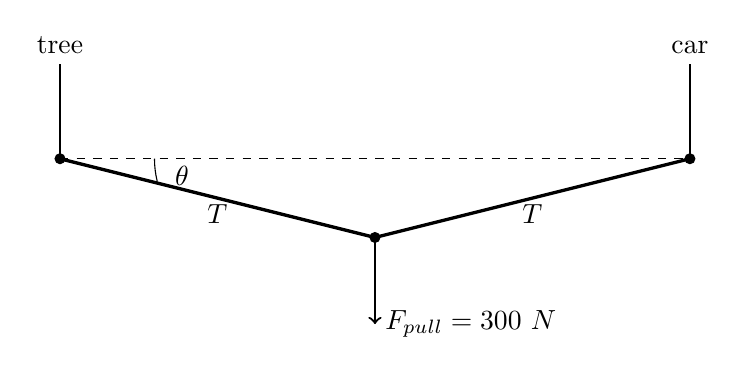
\begin{tikzpicture}[scale=1.0]
  % anchors
  \draw[thick] (0,0) -- (0,1.2) node[above]{tree};
  \fill (0,0) circle (2pt);
  \draw[thick] (8,0) -- (8,1.2) node[above]{car};
  \fill (8,0) circle (2pt);
  % straight (undeflected) line
  \draw[dashed] (0,0) -- (8,0);
  % deflected chain
  \draw[very thick] (0,0) -- (4,-1) -- (8,0);
  \fill (4,-1) circle (2pt);
  % pull force
  \draw[->, thick] (4,-1) -- (4,-2.1) node[right]{$F_\text{pull}=300~\text{N}$};
  % angle
  \draw (1.2,0) arc (180:194:1.2);
  \node at (1.55,-0.22) {$\theta$};
  \node at (2.0,-0.7) {$T$};
  \node at (6.0,-0.7) {$T$};
\end{tikzpicture}
\end{center}

  \begin{enumerate}[itemsep=2.7cm]
    \item Find the tension $T$ in the chain.
    \item The mechanical advantage on the car is $\text{MA}=\dfrac{T}{F_\text{pull}}=\dfrac{1}{2\sin\theta}$. Evaluate it.
    \item As the chain is pulled tighter and $\theta$ gets \emph{smaller}, what happens to the force on the car? Explain in one or two sentences, and state one practical danger.
  \end{enumerate}
  \vspace{1.4cm}
\newpage
%--- Problem 4: hydraulics (circle area, MA, PSI->kPa) ---
\item \textbf{Hydraulic lift.} A hydraulic lift has a small input piston of diameter $2.0~\text{cm}$ and a large output piston of diameter $30~\text{cm}$.

\begin{center}
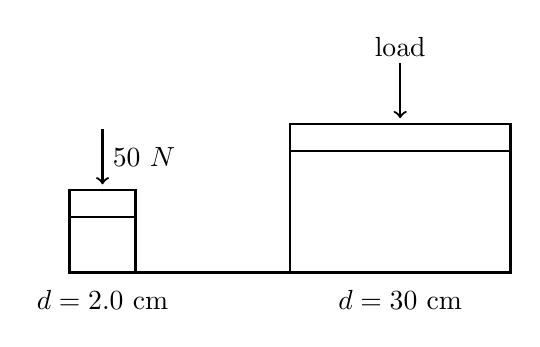
\begin{tikzpicture}[scale=0.7]
  \draw[thick] (0,0) rectangle (1.2,1.0);            % small cylinder
  \draw[thick] (0,1.0) rectangle (1.2,1.5);          % small piston
  \draw[->,thick] (0.6,2.6) -- (0.6,1.6) node[midway,right]{$50~\text{N}$};
  \draw[thick] (1.2,0) -- (4.0,0);                    % connecting tube bottom
  \draw[thick] (4.0,0) rectangle (8.0,2.2);          % large cylinder
  \draw[thick] (4.0,2.2) rectangle (8.0,2.7);        % large piston
  \draw[->,thick] (6.0,3.8) -- (6.0,2.8);
  \node at (6.0,4.1) {load};
  \node at (0.6,-0.5) {$d=2.0$ cm};
  \node at (6.0,-0.5) {$d=30$ cm};
\end{tikzpicture}
\end{center}

  \begin{enumerate}[itemsep=2.7cm]
    \item Find the area of each piston in $\text{cm}^2$ (use $A=\pi r^2$; the radius is half the diameter).
    \item Use Pascal's principle to find the mechanical advantage $\dfrac{A_\text{large}}{A_\text{small}}$.
    \item A force of $50~\text{N}$ pushes the small piston. Find the output force on the large piston.
    \item The system is rated for an operating pressure of $1500~\text{PSI}$. Convert this to $\text{kPa}$. Show one line of work using the unit factor $1~\text{PSI}=6.895~\text{kPa}$.
  \end{enumerate}
  \vspace{1.2cm}

\end{enumerate}

\end{document}
